\documentclass {CSEThesis}
% Standard packages
\usepackage{amsmath}        % Extra math definitions
\usepackage{graphics}       % PostScript figures
\usepackage{setspace}       % 1.5 spacing
% \usepackage{psfig,epsfig}
\usepackage{multicol}
\usepackage{subfigure}
\usepackage{hyperref}
\usepackage{epsfig,color}
\hypersetup{
    colorlinks=true,
    linkcolor=black,
    % filecolor=magenta,      
    urlcolor=blue,
}
 
\urlstyle{same}
% Custom packages
% \usepackage[first]{datestamp}   % Datestamp on first page of each chapter

\usepackage[utf8]{inputenc}
\usepackage[english]{babel}
\usepackage{minted}
\setminted{breaklines=true, tabsize=2, breaksymbolleft=}

\usepackage{color}
%===== page layout
% Define the side margins for a right-side page
% \insidemargin = 1.3in \outsidemargin = 0.9in
% Above margin is space above the header
% Below margin is space below footer
%\abovemargin = 1.5in \belowmargin = 0.05in


\btptitle = {Deep reinforcement learning(SLAM)} % { and } are needed around your name
\name = {Rajendra Singh}          % and other Fields. don't remove.
\rollno = {111601017}
\email = {111601017@smail.iitpkd.ac.in}
\guide = {Dr. Chandra Shekar }


\begin{document}

\begin{titlepage}
\begin{center}
\textheight 15.5in \textwidth 12.5in {\large\sf  \textbf{\the\btptitle}}\\[12ex]
{\small{\textsl{ \textbf{A Project Report Submitted \\
in Partial Fulfillment of the Requirements \\
for the Degree of \\
[3ex]\small \bf Bachelor of Technology}}}}\\
[16ex] \emph{by}
\\[2ex]
{\sf \sf \textbf{\the\name}\\
             (\the\rollno)}\\[1ex]
\emph{under the guidance of}\\[2ex]
{\sf \bf \the\guide} \\[7ex]

\vspace{1.2in}

 \begin{figure}[!h]
\centering
 
\includegraphics[width=0.15\textwidth]{IITPkdFullLogoColor}
 \end{figure}



{\small\bf DEPARTMENT OF COMPUTER SCIENCE AND ENGINEERING}  \\[1ex]
%{\small \bf{INDIAN INSTITUTE OF TECHNOLOGY PALAKKAD}}
%\\[2ex]
%
%  {\color{red} \hrule height 0.5ex}
% \vskip 1ex
% May \the\year 
\end{center}
\end{titlepage}



\raggedbottom
\doublespacing
\pagenumbering{roman}
\chapter*{\centering \underline{CERTIFICATE}}
\vskip 2ex \emph{\quad This is to certify that the work contained
in this thesis entitled ``\textbf{\the\btptitle}'' 
is a bonafide work of \textbf{\the\name}
(\textbf{Roll No. \the\rollno}), carried out in the Department of
Computer Science and Engineering, Indian Institute of Technology
Palakkad under my supervision and that it has not been submitted
elsewhere for a degree.} \vskip 15ex

\begin{flushright}
	\textbf{Your mentors name}\\
	Assistant/Associate Professor \\
	Department of Computer Science \& Engineering \\
	Indian Institute of Technology Palakkad
\end{flushright}
\hfill 
\hfill 






\chapter*{\centering Acknowledgements}
\quad I would like to express my special thanks of gratitude to my mentor \textbf{\the\guide} as well as our project coordinator \textbf{Albert sunny} who gave me the golden opportunity to do this wonderful project on the topic \textbf{\the\btptitle}, which also helped me in doing a lot of Research and I came to know about so many new things I am really thankful to them.
Secondly I would also like to thank my parents and friends who helped me a lot in finalizing this project within the limited time frame.



\tableofcontents 

\addcontentsline{toc}{chapter}{List of Figures} 
\listoffigures 

% \addcontentsline{toc}{chapter}{List of Tables} 
% \listoftables

\pagenumbering{arabic}
\def\headrulehook{\color{black}}      % Color the header rule

%========== Chapters
\typeout{}
\chapter{Introduction}
\pagenumbering{arabic}\hspace{3mm}

Write introduction.

\section{Section name}
1st Section

\section{2nd Section name}

2nd Section

\section{Organization of The Report}

You can write the about organization of your report in the following manner.

This chapter provides a background for the topics covered in this
report. We provided a description of wireless ad hoc networks, and
their applications. Then we described the network model that
represents the topology of wireless ad hoc networks \cite{Omar2016}. In this
chapter it is shown that the virtual backbone for wireless ad hoc
networks can be represented by a connected dominating set. We
explained clustering concepts and lastly the difference between
centralized and distributed algorithms are also discussed. The
rest of the chapters are organised as follows: next chapter we
provide review of prior works. In Chapter 3 and 4, we discuss our
new algorithms for constructing small backbones for ad-hoc
wireless network. And finally in chapter 6, we conclude with some
future works.


\cleardoublepage 
\typeout{}
\chapter{Simultaneous localization and mapping (SLAM)}

\section{Motivation}
Mobile robots are gaining significant relevance and starting to enter our daily life. For example, Vacuum cleaner,robotic lawnmower. Besides, they become more popular in the industry. Many companies started to use automated guided vehicles or mobile manipulators in their warehouses. Moreover, mobile robots are used in explorations of caves, pyramids, reefs or similar things. Another possible application of mobile robots in military operations where they could be used for transportation, reconnaissance or even fighting. The main request to a mobile robot obviously is mobility. The robot has to be capable of moving from its current pose, defined by its position and orientation, to a desired target configuration. In order to achieve this, it needs to find a valid collision-free path connecting the corresponding configurations. Moreover, there may be other demands to the path like to be as short, as fast or as safe as possible. If the robot wants to find such a path it needs access to several information. Firstly it needs information about itself such as its own size and its manoeuvrability. Furthermore, the environment including the current pose and the target pose have to be known. For this purpose mobile robots usually use a map. Now given this information path can be found. These paths can be calculated with several path planning algorithms. Planning algorithms usually work in discrete domains, which is why often trajectory optimization methods are used in the second step in order to smoother these paths. SLAM methods can create a map of an unknown environment and localize the robot in this map at once. That means they allow the robot to deal with any unknown environment. Therefore they are very popular and often used in mobile robotics. With SLAM there is no more need to create a map and hand it to the robot in order to navigate it since the robot develops its own.\cite{ustintern}




\section{Introduction}
Human beings get the information about their surrounding through vision, hearing the voice through ears, smelling through the nose and they do feel the strength of objects through touch. In general human beings get information about reality through senses. A robot cannot explore an unknown environment unless it is provided with some sensing sources to get information about the environment. There are different kinds of sensors used to make a robot capable of sensing a wide range of environments: Odometers, Laser range finders, Global Position System (GPS), Inertial Measurement Units (IMU), Sound Navigation and Ranging (Sonar) and cameras. The map of the environment is a basic need for a robot to perform actions like moving room to room, picking an object from one place and taking it to another one. To perform such actions, the robot should not only know about the environment but while it is moving it should also be aware of its own location in that environment. The aim to achieve is the navigation of the robot in a new and unknown environment by using the ROS. Robot builds the map, localizes itself on the map and performs navigation.
Simultaneous localization and mapping is a problem where a moving object needs to build a map of an unknown environment, while simultaneously calculating its position within this map. There are several areas which could benefit from having autonomous vehicles with SLAM algorithms implemented. Examples would be the mining industry, underwater exploration, and planetary exploration.\cite{ustintern}


\subsection{Formulation}
The SLAM problem, in general, can be formulated using a probability density function denoted \cite{ustintern}

\begin{mint}{python}
    p(xt, m|z1: t, u1:t )
\end{mint}

\begin{mint}{python}
'''
where, xt is  position of the vehicle at time t,
m       -  map,
z1:t    -  vector of all measurements(Observations),
u1:t    - vector of the control signals of the vehicle(control commands or odometry
'''
\end{mint}




\subsection{Data association}\\
Basically, the concept data association is to investigate the relationship between older data and new data gathered. In a SLAM context, it is of necessity to relate older measurements to newer measurements. This enables the process of determining the locations of landmarks in the environment, and thus this also gives information regarding the robot's position within the map. 
Simultaneous localization and mapping.\cite{ustintern}



\subsection{Loop closure}\\
The concept of loop closure in a SLAM context is the ability of a vehicle to recognize that a location has already been visited. By applying a loop closure algorithm, the accuracy of both the map and the vehicle's position within the map can be increased. However, this is not an easy task to perform, due to the fact that the operating environment of the vehicle could contain similar structural circumstances as previously visited locations. In that case, if the loop closure algorithm performs poorly, it could lead to a faulty loop closure, which could corrupt both the map as well as the pose of the vehicle within the map.\cite{ustintern}




\subsection{Full SLAM and online SLAM}\\
There are two different types of SLAM problems. The online SLAM problem of which only the current pose xt(x at time t) and the map m are expressed, given the control input u1:t and measurements z1: t. As well as the full SLAM problem which expresses the entire trajectory of the robot. The PDF of the full SLAM problem is denoted as p(x0: t, m|z1:t , u1:t ), where all the poses of the robot are considered, including its initial pose x0.




\subsection{General models for SLAM problem}
Challenge of SLAM is to compute the robots state xt and the map m depending on previous observations z0:t and control commands u0:t-1. For this to happen a motion model returning the current state xt depending on the previous state xt-1 and the last control command ut-1 is needed. The motion model is typically derived from the odometry data of the robot. Since odometry is sensitive to errors like non-round contours of the wheels, belt slip or inaccurate calibration this model is not deterministic. However, it can describe the belief of the state p(xt) as conditional probability 
p(xt) := P(xt |xt-1, ut-1)
Furthermore an observation model returning the current expected sensor output zt depending on the state xt and the map m has to be known. Due to inaccuracies of the sensors, this model is also not deterministic, but can be described as conditional probability 
p(zt) := P(zt |xt , m)
These models being non-deterministic means that everything we calculate using them will not be absolute. That implies that the SLAM problem can not be solved absolutely. It is not possible to compute the actual state or map. But what can be estimated is a belief over state and map represented by a probability. Assuming we know the motion and transition model of a certain robot and all previous states x0:t , the belief over the map m could be easily computed as 
p(m) := P(m|x0:t , z0:t , u0:t-1) 
Vice versa, if the map m and the models are known, the state xt can be estimated as 
p(xt) := P(xt |m, z0:t , u0:t-1)
But in the SLAM problem the robot knows neither its location nor the surrounding environment. And it is not just that both are unknown, in fact they depend on each other, which makes SLAM a chicken-egg-problem. The challenge is to compute the belief over the map m and the state xt simultaneously since they can not be estimated one after each other. Moreover, this has to be done carefully because wrong data association can lead to divergence. In fact there exist two different definitions of the SLAM problem. The first only seeks to recover the current pose xt and is formulated as 
p(xt , m) := P(xt , m|z0:t , u0:t-1)
This description is known as online SLAM. The other definition, which is called full SLAM, estimates the whole state trajectory x0:t as 
p(x0:t , m) := P(x0:t , m|z0:t , u0:t-1) 
Above two equations may seem impossible to solve at first. But since the solution of the SLAM problem is very significant for mobile robotics, it is a well-studied problem and there were several methods developed to solve it.\cite{ustintern}


\newline \begin{figure}[H]
    \centering
    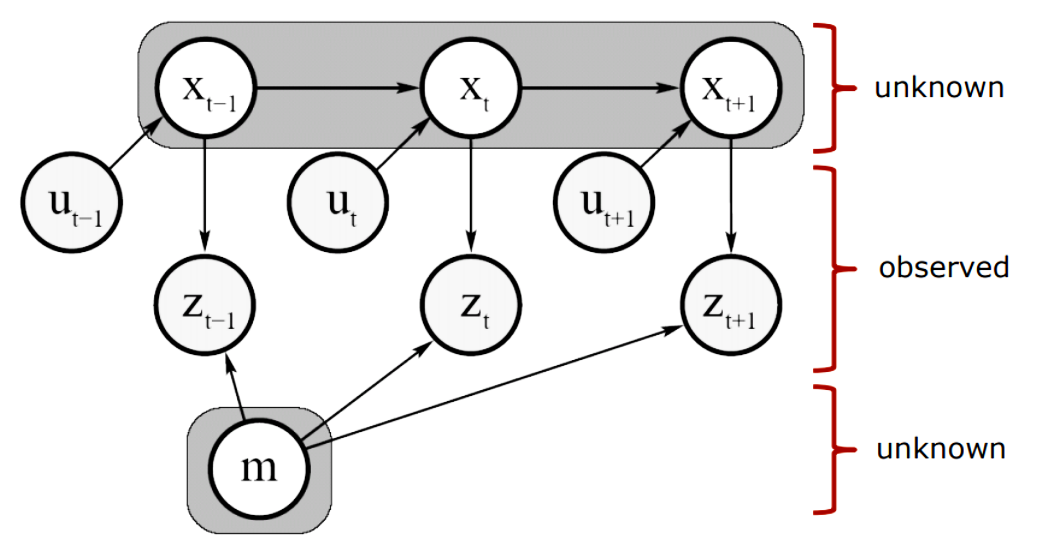
\includegraphics[width=0.5\textwidth]{images/slam.png}
    \caption{SLAM}
\end{figure}


\section{Implementation}


\subsection{Gmapping slam using lidar}
I used RPLidar A208 model to create map the environment. I implemented gmapping slam to create the map and tested the navigation on turtlebot burger model in gazebo simulation. Detailed description of which is as below:\cite{ustintern}
\newline \begin{figure}[H]
    \centering
    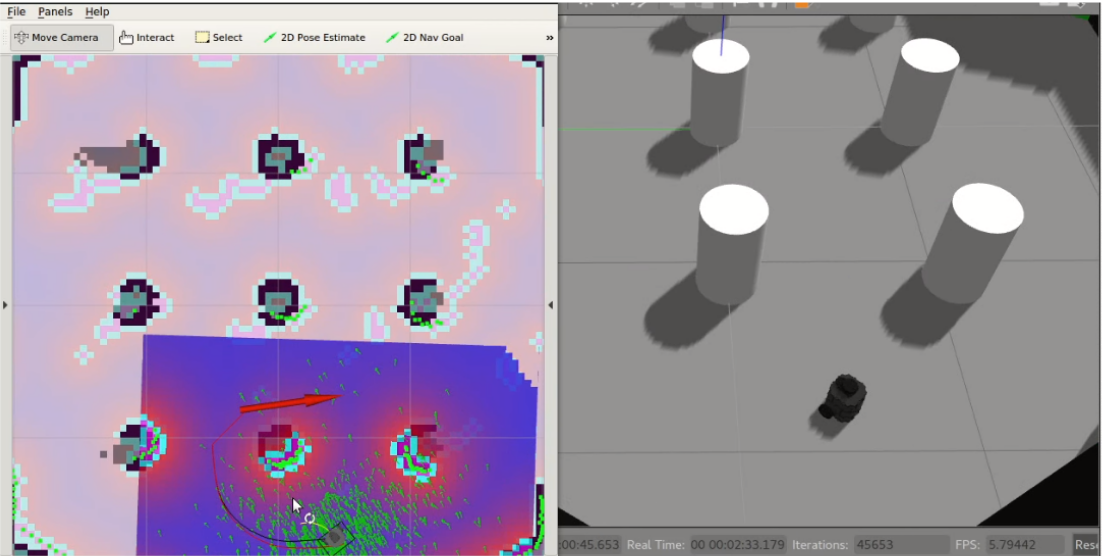
\includegraphics[width=1.0\textwidth]{images/gmapping.png}
    \caption{Gmapping using lidar}
\end{figure}
\begin{itemize}
    \item Firstly I create ros node to read the lidar data and publish scan message on /scan topic.
    \item Here we use the turtlebot burger model in gazebo, to get the relevant tf of robot.
    \item Instead of subscribing to the scan topic generated by gazebo model we subscribe our real robot lidar sensor.
    \item Now let create launch file for mapping where we do the following:            demo
    \begin{itemize}
        \item Launch the turtlebot world and spawn the burger model.
        \item Now we run the instance of the robot state publisher for getting relevant transforms.
        \item Load the urdf to robot description param.
        \item Launch lidar node.
        \item Now we run the slam\_gmapping node from gmapping package with appropriate base, odom and map frame.
        \item Launch the rviz node.
        \item Now we move the robot around using the teleop node, create the map.
        \item Once we’re happy with the generated map, we save it using the map\_saver node from map\_server pkg.
    \end{itemize}
    \begin{itemize}
    \item Now once we have the good map of environment, we navigate around the space: demo
        \item Here also we run the similar launch file as in mapping, just that we do not launch slam\_gmapping node.
        \item We launch the map\_server node for publishing the already saved map, as global map.
        \item We also run the instance of the acml node which will localise the robot in the surrounding environment, publish robot pose as covariance vector, which will improve over time.
        \item Then we run the move\_base node which is responsible for robot path planning. Here we used 2 types of DWAPlanner:
        \begin{itemize}
            \item Global planner : It is responsible for giving the global optimised path between start and destination pose.
            \item Local planner: It is responsible for planning the path locally for instance, when there also people moving in the same environment. In this case we can not navigate based on the global plan is based out one time static map.
        \end{itemize}
        \item Here our case we rviz gui tool to initial state estimation, and giving the goal.
    \end{itemize}
\end{itemize}


\subsection{RTAB-MAP slam using 3D Camera} demo
    I used intel realsense D435 to get the pointcloud data of real environment. This data was used to create the 3D map to environment using RTABMAP slam algorithm. Real-Time Appearance-Based Mapping(RTAB-Map) is a RGB-D, Stereo and Lidar Graph-Based SLAM approach based on an incremental appearance-based loop closure detector. The loop closure detector uses a bag-of-words approach to determinate how likely a new image comes from a previous location or a new location. When a loop closure hypothesis is accepted, a new constraint is added to the map’s graph, then a graph optimizer minimizes the errors in the map. A memory management approach is used to limit the number of locations used for loop closure detection and graph optimization, so that real-time constraints on large-scale environnements are always respected. RTAB-Map can be used alone with a handheld Kinect, a stereo camera or a 3D lidar for 6 DoF mapping, or on a robot equipped with a laser rangefinder for 3 DoF mapping. I followed these steps for creating 3d map of the environment:\cite{ustintern}
    \newline \begin{figure}[H]
        \centering
        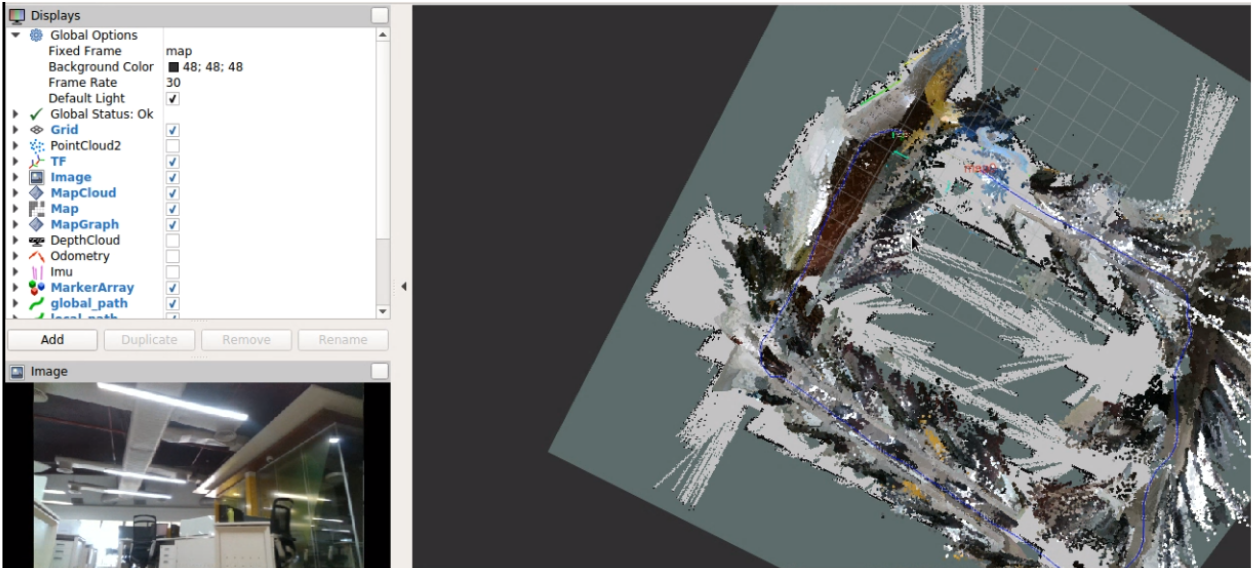
\includegraphics[width=1.0\textwidth]{images/rtabmap.png}
        \caption{RtabMap on AGV using lidar and 3D camera}
    \end{figure}
    \begin{itemize}
    \item First of we launch node which read the rgb and depth image from the 3d camera and publish as rostopic.
    \item We run rgbd\_sync node to sync these images if they aren't already.
    \item We can run the rtabmap is these two modes:
    \begin{itemize}
        \item Visual odom : This is feature based odometry, where we use the image feature to localise the robot in the environment. An RGBD odometry finds the camera movement between two consecutive RGBD image pairs. The input are two instances of RGBDImage. The output is the motion in the form of a rigid body transformation.
        \item Icp\_odom : Its use iterative closest point(icp) algorithm to get the odom data.
    \end{itemize}
    
    \item We use the lidar data along with pointcloud2 data to get more accurate mapping of the environment.
    \item Then run the rtabmap node with appropriate sensor topics, frames and parameter.
    \item For visualisation of the mapping we can either use rtabmapviz or rviz.
    \item Once we are happy with the obtained map, we stop the mapping. This will save the 3d map,poses and camera images .db file which can be used later during the navigation.
    \item We can also further do post processing on the obtained to map to further refine it.
\end{itemize}

Similar to the mapping we can also run the rtabmap in localisation mode where its will use previously generated map to localise in environment. Also we can give the goal pose directly through rviz path planning.


\section{Conclusion}
In this chapter studied various type of slam and its related terminology. We also implemented gmapping and RTABMAP slam. This chapter establish the base for future work where we will improve this algorithms usign reinforcement learning based algorithms.
% \end{document}
% \cleardoublepage 
\typeout{}
\chapter{Algorithm I}

give details of your algorithm

\section{Conclusion}
In this chapter, we proposed a distributed algorithm
for construction of xyz.
The complexity of this algorithm is $O(n \log n)$.
Next chapter presents
another distributed algorithm which has linear time 
complexity based on xyz.


\cleardoublepage 
\typeout{}
\chapter{Algorithm II}

The algorithm presented in previous chapter has $O(n)$ time 
complexity. We further propose another
distributed algorithm in this chapter based on xyz which has linear time 
complexity.

\section{Construction}

Write ...

\section{Improved Method}

Write...

\section{Conclusion}
In this chapter, we proposed another distributed algorithm for
XYZ. This algorithm has both time complexity of $O(n)$ where $n$
is the total number of nodes.  In next chapter, we conclude and
discuss some of the future aspects.


% \cleardoublepage 
% \clearpage
\typeout{}
\chapter{Conclusion and Future Work}

In this report, we successfully learnt about SLAM and Swarm Intelligence. We begin with understand various slam method. Then, we implement various RL algorithm(Q-learning, Sarsa, DQN) to solve the mountain car problem to understand these algorithm in depth. Later, we also used some of these algorithms to control the quad-copter. We show that how these method ease the process control compered to conventional method of pid tuning.\\
In the later part, studied various swarm algorithm and shown that how multiple robot together can perform most of the task better than any of individual robot in group can.\\

It seems we have build sufficient theoretically background and also have tested and varified our algorithm on simulated robots. Its high time we start implementing algorithm on hardware and further improve them. Hence in future, I will be working to implement this algorithms on hardware.\\
% \clearpage
\typeout{}

\newpage
\chapter*{References}
% \textit{\quad 
% 1.asdkf
% 2. sadfdsf
% }
1. OpenAI gym,  \url{https://gym.openai.com/}
\\2. ROS,  \url{http://wiki.ros.org/}
\\3. The Construct(ROS development studio), \url{https://rds.theconstructsim.com/}
\\4. My Rosject,  \url{http://www.rosject.io/l/ca1685c/}
\\5. My github repo,  \url{https://github.com/iamrajee/Slam_and_RL_BTP}
\\6. ARdrone simulation,  \url{https://github.com/AutonomyLab/ardrone_autonomy}
\\7. Pluto drone ros,  \url{http://wiki.ros.org/pluto_drone}
\\8. PID controller,  \url{https://en.wikipedia.org/wiki/PID_controller}




% \cleardoublepage 
\typeout{}
% \bibliographystyle{IEEEtran}
% \bibliography{btp}
\end{document}

